%*********************************************************************
% gdutthesis: 广东工业大学论文模板
% 2021/11/09 v0.1c
%
% 重要提示:
%   1. 请确保使用 UTF-8 编码保存
%   2. 请使用 XeLaTeX 或 LuaLaTeX 编译
%   3. 请仔细阅读用户文档和 Wiki
%   4. 修改、使用、发布本文档请务必遵循 LaTeX Project Public License
%   5. 不需要的注释可以尽情删除
%*********************************************************************
\documentclass[
  % type=doctor
  type=master
  % type=promaster
]{gdutthesis}

% 宏包在这里加载
\usepackage{siunitx}[=v2]
\usepackage{zhlipsum,lipsum}

\gdutsetup{
  style = {
    cover           = {true},
    % cover           = {false},
    % font            = {garamond},
    % font            = {libertinus},
    % font            = {lm},
    % font            = {palatino},
    font            = {times},
    % font            = {times*},
    cjk-font        = {fandol},
    % cjk-font        = {founder},
    % cjk-font        = {mac},
    % cjk-font        = {sourcehan},
    % cjk-font        = {noto},
    % cjk-font        = {windows},
    % cjk-font        = {none},
    bib-backend     = {bibtex},
    % bib-backend     = {biblatex},
    bib-resource    = {gdutthesis-template.bib},
    bib-style       = {numerical},
    % bib-style       = {author-year},
    fullwidth-stop  = {mapping},
    % fullwidth-stop  = {catcode},
    % fullwidth-stop  = {false},
    hyperlink       = {color},
    % hyperlink       = {border},
    % hyperlink       = {none},
    hyperlink-color = {default},
    % hyperlink-color = {autumn},
    % hyperlink-color = {business},
    % hyperlink-color = {classic},
    % hyperlink-color = {elegant},
    % hyperlink-color = {fantasy},
    % hyperlink-color = {material},
    % hyperlink-color = {science},
    % hyperlink-color = {summer},
    % hyperlink-color = {graylevel},
    % hyperlink-color = {prl},
  },
  info = {
    title           = {多旋翼飞行器导航与控制算法研究},
    title*          = {Research on navigation and control algorithm of multi-rotor aircraft},
    date            = {2022/5/25},
    author          = {邓正雄},
    author*         = {Deng Zhengxiong},
    supervisor      = {鲁仁全\qquad 教授},
    supervisor*     = {Prof. Lu Renquan},
    supervisor-two  = {none},
    supervisor-two* = {none},
    department      = {自动化学院},
    department*     = {Automation},
    major           = {控制科学与工程},
    student-id      = {2111904069},
    chairman        = {赵六\qquad 教授},
    degree          = {工程硕士},
    degree*         = {Master of Engineering},
    keywords        = {多旋翼, 状态估计, 控制, 校准},
    keywords*       = {multi rotor, state estimation, control, calibration},
    secret-level    = {none},
  }
}


\begin{document}

\begin{abstract}
  由于多旋翼飞行器具有体积小、机动性强、悬停能力强等优点,其在监视、搜索和救援等场景有很好的应用前景。
  在这些场景中,飞行器必须能够自主飞行,以尽量减少操作员的工作量。
  随着近年来机器人技术的快速发展,能够实现自主飞行的飞行器已经广泛应用于各种场景当中。
  但是,在传感器受干扰、使用低成本传感器情况下进行自主飞行会带来一些具有挑战性的工程问题。
  解决这些工程问题需要对估计、校准、控制等算法进行综合设计。
  其中,状态估计是自主飞行的首要和最关键的组成部分。
  本文提出了以状态估计为重点的方法和系统设计,使多旋翼飞行器能够在传感器信息受限及干扰情况下自主飞行。
  首先,我们提出了预测-修正-延时融合框架,以处理多频率多延时的传感器系统。
  然后,我们对每个传感器的特性进行研究,针对磁场干扰及运动加速度补偿进行优化处理,以提高系统的鲁棒性。
  其次,我们进一步优化了IMU校准算法,提高了IMU本身输出数据的精度。
  最后,我们整合了控制算法,形成一个完整的飞行控制系统。
  本文提供了大量的实验结果。
  最后,我们提出了未来的研究方向。
\end{abstract}

\begin{abstract*}
  Micro aerial vehicles (MAVs) are ideal platforms for surveillance and search and rescue due to their small size, superior mobility, and hover capability.
  In such missions, it is essential that the MAV is capable of autonomous flight to minimize operator workload.
  With the rapid development of robot technology in recent years, aircraft capable of autonomous flight has been widely used in various scenarios.
  Autonomous navigation in sensor interference, the use of low-cost sensors gives rise to challenging engineering
  problems.
  We require an integrated approach to estimation, calibration, and control to solve these engineering problems.
  Among these, state estimation is the first and most critical component for autonomous flight.   
  In this thesis, we present methodologies and system designs, with a focus on state estimation, that enable a light-weight off-the-shelf quadrotor MAV to autonomously navigate in the case of sensor information limitation and interference.
  We start by presenting a prediction-correction-delay fusion framework to deal with multi-frequency and multi-delay sensor systems.
  We then investigate the characteristics of each sensor and optimize the magnetic field interference and motion acceleration compensation to improve robustness.
  We further optimize the IMU calibration algorithm and improve the accuracy of IMU output data.
  Finally, we integrated the control algorithm into a complete flight control system.  	
  Extensive experimental results are presented throughout the thesis. 
  We conclude by proposing future research opportunities.
\end{abstract*}

\begin{notation}
  $E$ & 能量 \\
  $F$ & 推力
\end{notation}

\gduttableofcontents

\mainmatter

\gdutchapter{绪论}{Introduction}

\gdutsection{研究背景及意义}{Background and significance of research}
由于多旋翼飞行器具有体积小、机动性强、悬停能力强等优点,其在监视、搜索和救援等场景有很好的应用前景。
在这些场景中,飞行器必须能够自主飞行,以尽量减少操作员的工作量。
随着近年来机器人技术的快速发展,能够实现自主飞行的飞行器已经广泛应用于各种场景当中,如航空摄影、交通运输和智能农业。
除了上述应用场景外,在人员和地面机器人难以接近或危险复杂环境中,飞行器在监视、搜索和救援任务中具有巨大的潜力。
在这样的环境中,飞行器作业的主要挑战是传感器干扰和传感器本身数据精度低。
传感器干扰包括但不限于气压计干扰、磁场干扰、GPS信号异常。
由于使用低成本的传感器,传感器本身的数据精度限制了导航系统的精度。
到目前为止,研发一个多旋翼飞行器,并能够在这样的环境中快速自主飞行,仍然会带来挑战性的工程问题,需要对估计、校准、控制等算法进行综合设计。
因此,本文将对状态估计、校准和控制这三个问题进行研究。
其中,状态估计是自主飞行的首要和最关键的组成部分。

\gdutsection{国内外研究现状}{Analysis of the research status at home and abroad}
近年来,人们对应用在多旋翼飞行器的导航与控制系统进行了广泛的研究。
我们首先回顾了多旋翼飞行器发展过程中出现的一些研究问题。
我们在本节回顾关于每个问题及其相关领域的文献。
接下来我们对估计、校准、控制三个问题进行回顾。

\gdutsubsection{传感器融合}{Sensor fusion}
估计一个刚体的状态(即位置和姿态)是机器人鲁棒和高性能控制的关键要求。
机器人的状态估计是一个非线性的问题,使用的传感器通常包含了非高斯噪声\cite{baldwin2009inertial}。
一种标准的方法是使用扩展的随机线性估计技术\cite{lefferts1982kalman,barshan1995inertial}。
另一种方法是使用确定性互补滤波器和非线性观测器设计技术\cite{zimmermann1992high,baerveldt1997low,vik2001nonlinear}。
在随机线性估计技术中,应用于姿态估计问题的主要算法是扩展卡尔曼滤波(EKF)型方法。
粒子滤波器也被认为是处理非线性的一种方法\cite{cheng2004particle}。
由于状态空间的非线性而遇到困难,EKF表现出非鲁棒性和不稳定性\cite{crassidis2007survey}。
相反,非线性观测器利用基础几何来解释问题本质中的非线性。
因此,非线性观测器相比于EKF鲁棒性更强,并具有可证明的几乎全局稳定的性质\cite{thienel2003coupled,mahony2008nonlinear,lageman2009gradient,hua2010attitude,vasconcelos2010nonlinear}。
对于姿态问题,Mahony等人利用所有旋转的特殊正交群SO(3)的基本李群结构推导了一个互补非线性姿态观测器,并证明了误差系统的几乎全局稳定性\cite{mahony2008nonlinear}。
磁场干扰会影响横滚角和俯仰角的估计。
Hua等人考虑了输入信号的解耦,以确保滚转和俯仰估计不受磁场干扰的影响,这代表了显式互补滤波器标准实现的一个重要修改,以提高姿态估计的整体质量\cite{hua2011nonlinear}。
大多数现有的姿态观测器/滤波器都依赖于小加速度假设(即$\dot{v}<<g$),因此重力方向测量可以近似于加速度计测量。
然而,对于许多垂直起降飞行器在快速运动中,飞行器的线性加速度通常是较大的,可能会在姿态估计上产生很大的误差。
对于较大的线性加速度,可以将GPS线速度的测量值与加速度计的测量值相结合来估计飞行器的加速度,从而提高姿态估计的精度。
Hua等人提出了GPS辅助姿态观测器\cite{hua2010attitude}。
以上提到的所有的观测器设计方法都要求对系统的当前输出和输入进行无延迟测量。
然而,在许多实际场景中,系统输出的测量值具有延时(与系统的理想输出比较),而系统输入的测量值可以看作没有延时。
例如,GPS提供的线速度(输出)测量值通常相对于飞行器的实际速度有延时的。
由于各种环境影响和传感器内部处理的延时,延时可以是几百毫秒(甚至半秒)\cite{kingston2004real}。
相比之下,IMU提供的机体角速度和线加速度的测量值几乎是瞬时的。
众所周知,测量延时会对观测器或滤波器的稳定性和鲁棒性产生负面影响,并降低其性能\cite{battilotti2015nonlinear}。
在估计问题中,解决传感器延时问题的经典方法是修改其修正项,使每个延时测量值与相应的后向时移估计值进行比较。
Khosravian等人提出了一种级联观察器-预测器方法来处理李群SO(3)上姿态估计的传感器延时问题\cite{khosravian2016state}。
作者利用李群SO(3)的特定代数结构,证明了误差系统的指数收敛性。
继Mahony在SO(3)上的工作之后,Baldwin等人提出了直接在SE(3)上使用全状态反馈和已知特征测量的互补观测器\cite{baldwin2007complementary}。
据本人所知,针对多频率多延时的传感器系统以及传感器异常处理,目前的方法不能很好地解决鲁棒性和安全性问题。

\gdutsubsection{传感器校准}{Sensor calibration}
IMU(惯性测量单元)是机器人工程中非常流行的传感器。
目前,IMU已被广泛用于惯性导航\cite{jekeli2012inertial}、姿态估计\cite{mahony2008nonlinear}、视觉惯性导航\cite{baldwin2009inertial},以及智能手机设备\cite{li2013real}。
机器人工程中使用的IMU通常是基于MEMS(微机电系统)技术。
IMU由一个加速度计和一个陀螺仪组成。
有些IMU还会加入磁力计。
对于一个理想的IMU,三轴传感器应该具备相同的三维正交敏感轴,比例因子应该将每个传感器测量的数字量转换为真实的物理量(如加速度和角速度)。
实际上,基于MEMS的低成本IMU误差通常包括不精确的尺度、传感器敏感轴不对齐和零偏的影响。
IMU校准指的是辨识这些物理量的过程。
IMU校准的传统方法是通过使用特殊的机械平台来完成的,如机器人机械手。
具体操作是以已知的旋转速度移动IMU到精确控制的姿态上\cite{hall2000case}。
在每个姿态上,加速度计的输出与预先计算的重力向量进行比较,而在旋转期间,陀螺仪的输出与预先计算的旋转速度进行比较。
然而,用于校准的机械平台通常非常昂贵,导致校准成本往往超过IMU的硬件成本。
Kim等人提出了一种利用基于标记的光学跟踪系统进行标定的方法,GPS读数用于校准初始偏差和非正交误差\cite{kim2004initial}。
显然,这些方法的精度非常依赖于所采用的运动参考的精度(即运动捕捉系统或GPS)。
多位置法最早是由Lotters等人提出的\cite{lotters1998procedure}。
Lotters等人提出,利用静态加速度的大小必须等于重力的大小这一事实,来校准加速度计的零偏和尺度。
该技术在文献\cite{syed2007new}中得到了扩展,增加了加速度计轴正交参数。
他们提出的陀螺仪误差模型与加速度计的误差模型相似,但这种情况下的校准流程需要单轴转台提供强大的转速信号,以提供较高的校准精度。
但是,这些方法有以下不足:需要一个机械设备,两个传感器是独立校准的,传感器之间的不对齐无法被检测到。
Fong等人提出了两种不需要任何外部机械设备的校准方案\cite{fong2008methods}。
与之前的方法类似,作者利用重力向量幅值的局部稳定性对加速度计进行标定,然后将标定后的加速度计感知到的重力向量与通过角速度积分得到的重力向量进行比较,得到陀螺仪的标定结果。
在文献\cite{cheuk2012automatic}中,作者还探讨了磁场的局部稳定性。
Hwangbo等人提出了一种基于迭代矩阵分解的自校准技术\cite{hwangbo2013imu}。
作者用重力作为加速度计的参考,用相机作为陀螺仪的参考。
Tedaldi等人在多位置法的基础上进行改进,提出了一种鲁棒且易于实现的方法来校准IMU,无需任何外部设备\cite{tedaldi2014robust}。
作者在优化算法内自动估计静态区间分割的阈值。
我们在Tedaldi工作的基础上,对最优阈值的算法进行修改。

\gdutsubsection{控制}{Control}
在获得了飞行器的状态后,我们可以使用各种现有的控制策略使飞行器稳定飞行。
线性控制器,如PID控制器或LQR控制器,被广泛应用于多旋翼飞行器中\cite{hoffmann2007quadrotor,castillo2004stabilization,nice2004design}。
基于飞行器工作接近悬停状态的假设下,对于低速运行、加速度变化小的飞行器,可以使用线性控制器。
针对四旋翼无人机在饱和位置下的线性化动力学问题,Guenard等人设计了一种非线性控制器\cite{guenard2005dynamic}。
文献\cite{bouabdallah2005backstepping}中应用了反步和滑模技术。
因为这些控制器是基于欧拉角设计的,它们在表示多旋翼飞行器复杂的旋转运动时表现出奇点,从而从根本上限制了它们跟踪轨迹的能力。
基于李群上的刚体动力学描述,Lee等人设计了一种应用在四旋翼飞行器的几何控制器,并证明了几乎全局稳定性\cite{lee2010geometric}。
对于包含大姿态变化的运动,文献\cite{lee2010geometric}的控制器是更合适的选择。

\gdutsection{实验平台概述}{Overview of Experimental Platforms}
我们研究的一个关键部分是对提出的算法和系统进行实验验证。
为此,我们开发了适合实验目的的飞行器平台。
我们的飞行器平台(\autoref{fig:platform})是使用现成的组件构建的。
\begin{figure}[htbp]
	\centering
	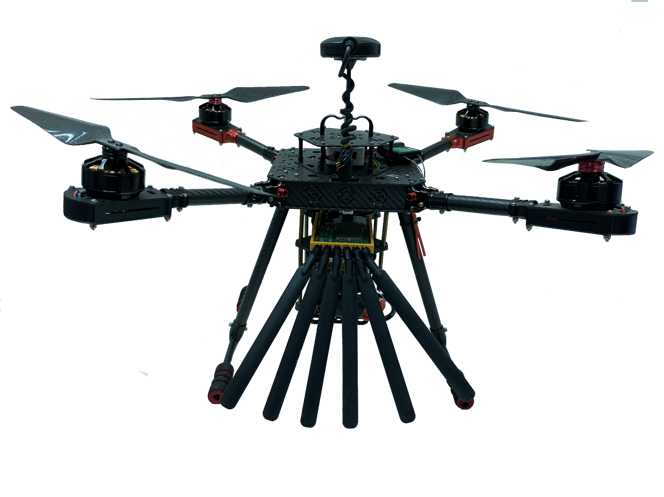
\includegraphics[width=0.7\textwidth]{platform.png}
	\bicaption{实验平台}{Experimental platform}
	\label{fig:platform}
\end{figure} 
实验平台上安装了一个飞控板(\autoref{fig:AutoPilotboard})。
我们在这个飞控板上实现我们的算法。
飞控板由IMU、磁力计、气压计和用户可编程的STM32微控制器组成。
\begin{figure}[htbp]
	\centering
	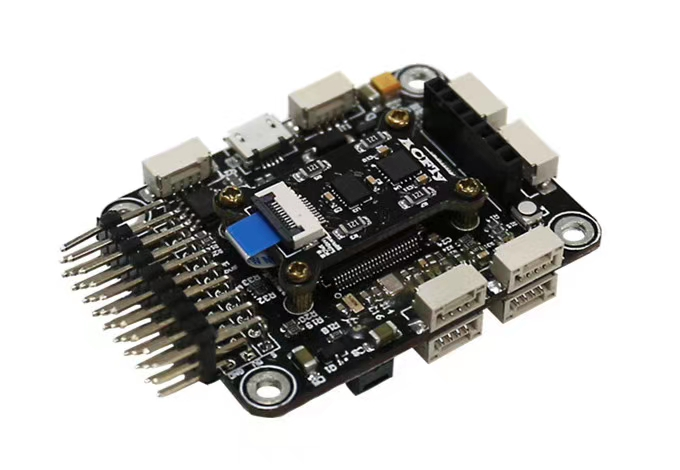
\includegraphics[width=0.7\textwidth]{acfly.jpg}
	\bicaption{飞控板}{AutoPilot board}
	\label{fig:AutoPilotboard}
\end{figure}
微控制器采用STM32H743VIT6(\autoref{fig:STM32H743VIT6}),主频高达480M,有16Kb的L1级缓存Cache,1M内存,2MFlash,支持硬件双精度浮点运算。
\begin{figure}[htbp]
	\centering
	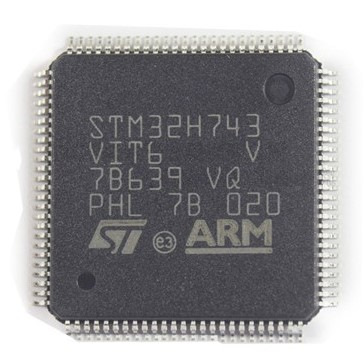
\includegraphics[width=0.3\textwidth]{St-Semiconductor-Chips-Electronic-Component-Lqfp-100-Stm32h743vit6.jpg}
	\bicaption{STM32H743VIT6}{STM32H743VIT6}
	\label{fig:STM32H743VIT6}
\end{figure}
IMU芯片采用BMI088(\autoref{fig:BMI088})。
BMI088是一款高性能六轴惯性测量单元,具有高振动稳定性,专为无人机和机器人应用而设计。
BMI088具有出色的抗振性和抑制能力,可在较大的温度变化下保持稳定。
BMI088的加速度计量程最大是24g,陀螺仪的最大量程是2000°/s。
即使在大震动环境下也不会超量程。
\begin{figure}[htbp]
	\centering
	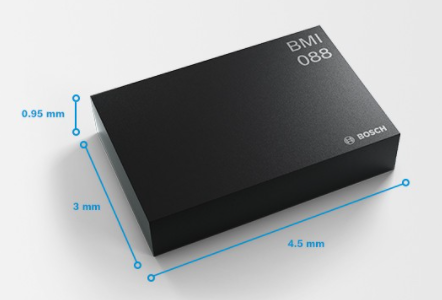
\includegraphics[width=0.5\textwidth]{屏幕截图 2022-03-30 151212.png}
	\bicaption{BMI088}{BMI088}
	\label{fig:BMI088}
\end{figure}
磁力计采用AK8975,气压计采用SPL06。
对于位置传感器,我们使用ublox的GPS模块。
本文中讨论的所有算法都是用C++实现,运行在上文提到的飞控板上。

\gdutchapter{传感器融合}{Sensor fusion}
本章介绍了我们开发的一种适用于多旋翼飞行器的传感器融合算法,使用IMU作为主要传感器。我们感兴趣的是在飞行器平台上运行的状态估计算法,这种应用场景对于传感器融合有不一样的要求。因此,我们针对这些系统需求处理传感器融合、异常处理等问题。

我们注意到,这个课题已经有很好的研究成果\cite{mahony2008nonlinear,hua2010attitude,khosravian2016state}。我们的工作与现有成果之间的主要区别在于,我们的系统整合了现有成果的方法,具有很强的鲁棒性。我们确保该系统能够在大震动、高机动环境、磁场干扰环境中稳健运行,在这些环境中,依赖单一现有成果的算法是不可行的。我们给出了各种环境下的实验结果,要求系统在一段较长的时间内无故障运行。
\begin{figure}[htbp]
	\centering
	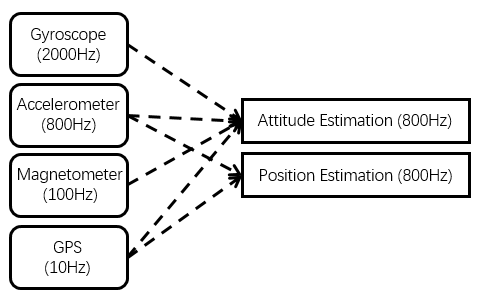
\includegraphics[width=0.7\textwidth]{state estimation.png}
	\bicaption{状态估计框架图}{Diagram of state estimation}
	\label{fig:stateestimation}
\end{figure} 

在本章中,我们将重点讨论系统中使用的状态估计方法(\autoref{fig:stateestimation})。我们将介绍由这些方法支持的系统飞行测试结果。我们注意到,自主飞行需要仔细地集成其他重要模块,如控制、校准等。这些模块的讨论放到后面两章。这些模块作为通用模块,以支持整个系统的运行。

\gdutsection{状态估计}{State estimation}
我们工作的核心是一个可靠的估计模块,该模块使用GPS、低成本的IMU和磁力计输出姿态、位置和速度。我们注意到,基于磁力计及GPS的偏航角估计较为特殊,因此,我们提出了一种解耦估计器设计。

我们将世界坐标系记为$\left\{ W \right\}$,将机体坐标系记为$\left\{ B \right\}$,将世界坐标系和机体坐标系中的向量分别定义为$(\cdot)^w$和$(\cdot)^b$。我们感兴趣的是世界坐标系中飞行器的姿态、位置和速度,其定义为
%\begin{equation}\label{eq:vector}
%\begin{bmatrix}
%	p^w_x & p^w_y & p^w_z & v^w_x & v^w_y & v^w_z & \phi^w & \theta^w & \psi^w
%\end{bmatrix}
%\end{equation}
$[p^w_x , p^w_y , p^w_z , v^w_x , v^w_y , v^w_z , \phi^w , \theta^w , \psi^w]$。
其中$p^w_x$、$p^w_y$和$p^w_z$是三维位置,$v^w_x$、$v^w_y$和$v^w_z$是三维速度,$\psi^w$、$\theta^w$和$\phi^w$是偏航角、俯仰角和横滚角,表示经过ZYX欧拉角转换后从机体坐标系到世界坐标系的旋转。因此,我们有旋转矩阵表示
\begin{equation}\label{eq:rotationmatrix}
	R_{b}^{w}=R(\psi^w)R(\theta^w)R(\phi^w)
\end{equation}

我们使用基于多传感器融合的状态估计方法来估计三维姿态、位置和速度。一种带延时观测的显式互补滤波器(ECF)将IMU数据与GPS融合,以提供横滚角($\phi^w$)和俯仰角($\theta^w$)的估计。解耦估计器将陀螺仪数据、磁力计数据和GPS融合,以提供偏航角($\psi^w$)的估计。一种带延时观测的三阶互补滤波器融合IMU和GPS数据输出三维位置和速度。

\gdutsubsection{横滚角、俯仰角估计}{Roll and pitch estimation}
直接安装在机体的惯性测量单元作为横滚角和俯仰角估计的主要信息来源。惯性测量单元(英文:Inertial measurement unit,简称IMU)是测量物体三轴姿态角(或角速率)以及加速度的装置。一般的,一个IMU内会装有三轴的陀螺仪和三个方向的加速度计,来测量物体在三维空间中的角速度和加速度,并以此解算出物体的姿态。

陀螺仪测量的是$\left\{ B \right\}$相对于$\left\{ W \right\}$的角速度,投影在机体系$\left\{ B \right\}$。
\begin{equation}\label{eq:gyromodel}
	\Omega^y=\Omega+b+\mu
\end{equation}
其中$\mu$表示加性测量噪声,$b$表示陀螺零偏。
姿态估计的第一步是将陀螺仪测量的角速度积分成陀螺仪的姿态。在早期的惯性导航应用中,因为计算机计算能力有限,人们曾经使用双速度积分法:高速一阶积分和中速高阶积分,从而在保证积分精度的前提下降低计算量\cite{savage1998strapdown}。在现在IMU的低精度应用中,一般单片机的计算性能足以保证在IMU的测量带宽内使用最精确的积分方法,因此我们没有必要讨论双速度积分法。在本文中,我们不考虑地球自身的旋转和地球的曲率,因此只限于小范围内的IMU的应用。陀螺仪积分出的姿态短时间内是准确的,但长时间后因为漂移误差精度会大幅下降\cite{钱华明2010基于}。

加速度计测量物体的比力,即去掉重力后的整体加速度或者单位质量上作用的非引力。
\begin{equation}\label{eq:accmodel}
	a=R^T(\dot{v}-g)+b_a+\mu_a
\end{equation}
其中$\mu_a$表示加性测量噪声,$b_a$表示加速度零偏,$\dot{v}$是世界系的加速度。
三轴加速度计的原理能够用来测量角度。在没有外力作用的情况下,加速度计能够精确地测量俯仰角和滚转角,且没有累积误差。由于加速度计本身的特性,加速度计解算的姿态很灵敏,非常容易受到振动以及运动加速度的影响\cite{赵翔2012基于}。

\gdutsubsection{偏航角估计}{Yaw estimation}
磁力计提供周围环境磁场的测量值。
\begin{equation}\label{eq:magmodel}
	m=R^T m^w+B_m+\mu_m
\end{equation}
其中$m^w$为在世界系的地球磁场矢量,$B_m$为局部磁场干扰,$\mu_m$为测量噪声。对于磁力计的读数,$\mu_m$通常是相当小的,但是,局部磁场干扰$B_m$可能是非常大的,特别是如果传感器被放置在电机的电源线附近。多旋翼飞行器通用的无刷电机在运转的时候就会产生变化的磁场,和地磁场叠加之后,通过这个有偏差的地磁向量作为参考去计算所得到的偏航角是不准确的,目前没有很好的办法去解决磁场干扰问题\cite{梅玲玉2019基于}。

\gdutsubsection{位置速度估计}{Position and velocity esitimation}
卫星导航系统(Global Navigation Satellite System, GNSS)是覆盖全球的自主地利空间定位的卫星系统,允许小巧的电子接收器确定它的所在位置(经度、纬度和高度),并且经由卫星广播沿着视线方向传送的时间信号精确到10米的范围内。在户外环境中,GPS通常用于提供位置、世界系的速度和航向角。GPS系统由一个24颗卫星组成的星座组成,这些卫星连续不断地围绕地球运行,高度为20180公里。GPS接收器的位置是通过观测卫星发送的信号的飞行时间来确定的,并被接收器探测到。如果接收机有准确的时间信息,则至少需要三个卫星信号来确定接收机的位置。然而,对于低成本的GPS接收器,也必须接收到定时信息,这需要至少4个卫星信号。存在各种各样的因素影响着GPS的估计。主要的误差来源包括卫星轨道数据不准确、卫星时钟不准确、信号通过电离层时的可变延迟、地球表面附近的天气状况以及来自附近建筑物和山脉的多径反射。GPS总体偏差约为5-10m。现代GPS接收机利用接收信号载波相位的多普勒频移来估计航向角和对地速度\cite{wendel2006integrated}。

\gdutsection{基于ECF的传感器融合}{ECF-based sensor fusion}
针对飞行器应用开发从业人员,我们希望设计一个模块化、容易扩展的传感器融合观测器。这意味着当我们需要增加或删除传感器时需要数学推导和编程的工作量应该是最小的。接下来我们将对目前流行算法的优缺点进行分析,以引出我们设计的融合框架。

一个标准的方法是使用扩展的随机线性估计技术\cite{lefferts1982kalman,barshan1995inertial}。另一种方法是使用确定性互补滤波器和非线性观测器设计技术\cite{zimmermann1992high,baerveldt1997low,vik2001nonlinear}。对于我们考虑的低成本、轻量化系统,线性滤波技术已被证明在应用场景中鲁棒性不强\cite{roberts2003low},而线性单输入单输出互补滤波器在实践中经常被使用\cite{saripalli2003tale,corke2004inertial}。前人关于非线性姿态观测者的研究有一个不足的地方是计算开销大,而且所构造姿态的误差较大。对于上述缺点,显式互补滤波器不需要对姿态进行在线代数重构。因此,该观测器非常适合在嵌入式硬件平台上实现。此外,对于不同的传感器数据的信任度可以在观测器响应中设置权重,这一特性允许开发人员根据传感器特定的噪声特性进行调整。最后,基于EKF的线性观测器方法在初始误差大时可能引起非常大的误差,而基于非线性控制方法的设计可以做到全局收敛。因此,我们采用基于ECF的非线性观测器的方法\cite{mahony2008nonlinear}。

\gdutsubsection{基于ECF的标准实现}{Standard implementation based on ECF}
姿态估计的目标是为估计量$\hat{R}(t)\in SO(3)$提供一组动力学方程来使得误差旋转矩阵$\widetilde{R}(t)\rightarrow I_3$。飞行器的姿态运动学方程为
\begin{equation}\label{eq:kinematics}
	\dot{R}=R\Omega_{\times}=(R\Omega)_{\times}R
\end{equation}
其中,$\Omega$是机体角速度。作者所提出的观测器方程直接作为一个运动学系统用于姿态估计。此观测器运动学包括基于测量的预测项和由误差导出的修正项。记$\hat{R}$表示对飞行器姿态$R$的估计。观测器的一般形式是
\begin{equation}\label{eq:passivefilter}
	\dot{\hat{R}}=\hat{R}(\Omega_{\times}+k_P \mathbb{P}_a(\widetilde{R}))
\end{equation}
其中,$k_P>0$。观测器框架如\autoref{fig:DiagramECF}所示。
\begin{figure}[htbp]
	\centering
	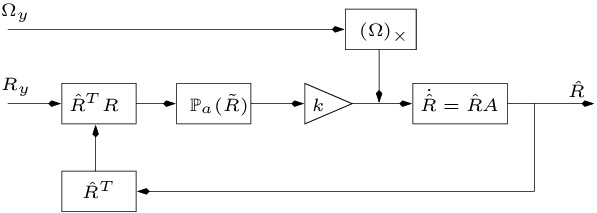
\includegraphics[width=0.7\textwidth]{Block-diagram-of-the-simplified-form-of-the-passive-complementary-filter.png}
	\bicaption{显式互补滤波框架图}{Block diagram of explicit complementary filter}
	\label{fig:DiagramECF}
\end{figure}
对于$\mathbb{P}_a(\widetilde{R})$,我们可以使用欧拉角相减,DCM或四元数相乘来获取姿态的误差,这样的方法都有一个缺点,那就是需要通过加速度计和磁力计的测量计算出一组姿态。虽然常用的方法比较成熟,但也有一些问题,比如欧拉角法存在奇异点(如在俯仰角90度时),DCM和四元数的TRIAD或QUEST等方法又需要额外的计算。ECF的突出贡献之一就是直接利用加速度计和磁力计的测量值,利用和惯性空间向量的叉乘,简单地就获得了姿态的误差。如下观测器是ECF的标准形式
\begin{equation}\label{eq:Explicitfilter}
	\begin{aligned}
	\dot{\hat{R}}&=\hat{R}((\Omega^y - \hat{b})_{\times}+k_P (\omega_{mes})_{\times})\\
	\dot{\hat{b}}&=-k_I \omega_{mes}\\
	\omega_{mes} &\coloneqq \sum_{n=1}^{n} k_i v_i \times \hat{v}_i	
	\end{aligned}
\end{equation}
其中$k_P$,$k_I$,$k_i$是任意非负的观测器增益。注意到姿态$\hat{R}$是整个观测器的输出。在文献\cite{mahony2008nonlinear}中对观测器(\autoref{eq:Explicitfilter})进行了广泛的研究,表明姿态和零偏能做到指数收敛(理论和实验)。该滤波器具有互补的特性,利用陀螺仪信号的高频部分和磁力计、加速度计的低频部分\cite{mahony2008nonlinear}。与这些信号相关联的截止频率由增益$k_P$,$k_I$,$k_i$决定。

用于表示旋转的单位四元数在代码实现中具有较高的效率,是实现$SO(3)$群运算的常用方法。上述观测器的四元数表示如下
\begin{equation}\label{eq:quatfilter}
	\begin{aligned}
	\dot{\hat{q}}&=\frac{1}{2} \hat{q} \otimes \mathbf{p}(\Omega_y - \hat{b} + k_P \omega_{mes})\\
	\dot{\hat{b}}&=-k_I \omega_{mes}\\
	\omega_{mes} &\coloneqq \sum_{n=1}^{n} k_i v_i \times \hat{v}_i	
\end{aligned}
\end{equation}

如果飞行器配备了GPS系统,估计速度和位置是一个简单的过程。在这种情况下,位置运动学是线性的,可以使用线性滤波器。记$\hat{p}$表示位置的估计,$\hat{v}$表示速度的估计。给出了一个简单的线性滤波器
\begin{equation}\label{eq:posfilter}
	\begin{aligned}
		\dot{\hat{p}}&=\hat{v}-k_x (\hat{p}-p_{GPS})\\
		\dot{\hat{v}}&=\hat{R}^T a - g e_3 - k_v (\hat{p}-p_{GPS})\\	
	\end{aligned}
\end{equation}
其中增益$k_x,k_v > 0$。只要姿态估计是准确的,这个滤波器具有很强的鲁棒性。此观测器可以很容易地加上加速度计的零偏估计。并且可以使用卡尔曼滤波去调节$k_x$和$k_v$。在实际应用中,对于微型飞行器系统,测量的噪声特性非常差,因此通常最好使用恒定增益滤波器,而不是引入附加的复杂性和潜在的不稳定性的Riccati方程与卡尔曼滤波器。

\gdutsubsection{使用GPS辅助的姿态观测器设计}{GPS-aided attitude observers}
大多数现有的姿态观察器/滤波器都依赖于小加速度假设($\dot{v}\approx 0$),因此重力方向测量可以近似于上一小节中讨论的加速度计测量。然而,对于许多飞行器都有高速运动的场景,会产生比较大的线性加速度,姿态估计器的输出可能会有较大的误差。对于较大的线性加速度,可以将GPS线速度的补充测量与加速度计的测量相结合来估计飞行器的加速度,从而提高姿态估计的精度。基于ECF的使用GPS辅助的姿态观测器被提出\cite{hua2010attitude}。值得注意的是,文中提出的观测器不能保证从磁场测量中对横滚角和俯仰角估计的解耦。

我们使用直接补偿的方法。只要与飞行器惯性运动相关的加速度分量得到补偿,加速度计的数据也可以使用。最简单的方法是使用绝对测量信号GPS来估计飞行器的加速度
\begin{equation}
	a_{CTD}=a_{IMU}-\hat{R}^T \dot{v}_{GPS}
\end{equation}
其中$a_{CTD}$是修正后的加速度。在这种情况下,满足$a_{CTD} \approx R^T e_3$,$a_{CTD}$能提供准确的姿态信息。值得注意的是,在上文提出的互补滤波器中,只需要$a_{CTD}$的低频成分。因此,GPS速度的一阶导数$\dot{v}_{GPS}$中的噪声影响较小。

\gdutsubsection{处理耦合问题}{Handling coupling issues}
在补偿了运动加速度后,使得假设$a_{CTD} \approx R^T e_3$成立,在这种情况下我们依然可以使用显式互补滤波器的标准实现(\autoref{eq:Explicitfilter}),我们这里再将修正项单独拿出来讨论
\begin{equation}
\omega_{mes} \coloneqq k_1 u_B \times \hat{u}_B + k_2 m_B \times \hat{m}_B	
\end{equation}
其中,增益$k_{1,2}>0$,$u_B = a_B / g$,$u_I = e_3$,$\hat{u}_B = \hat{R}^T u_I$,$\overline{m}_B = m_B / \left| m_I \right|$,$\overline{m}_I = m_I / \left| m_I \right|$,$\hat{\overline{m}}_B = \hat{R}^T \overline{m}_I$。然而,研究人员已经认识到这个标准实现存在一些耦合问题,这些问题在文献\cite{hua2013implementation,hua2011nonlinear,martin2007invariant}中已经进行了深入的讨论。

磁场干扰和零偏会影响横滚角和俯仰角的估计。在实际应用中,特别是在使用电机作为执行器的小型飞行器中,较大的磁场干扰几乎是不可避免的,导致$m_B$和$R^T m_I$之间存在较大的时变误差。这不仅会导致偏航角的估计误差很大,而且还会导致横滚角和俯仰角估计产生误差。
滚转角,俯仰角和偏航角估计的动力学方程是高度耦合的。这意味着偏航角的估计会较大地影响着横滚角和俯仰角的估计。在实际应用中,重力矢量和地球磁场矢量(即$e_3$和$m_I$)可能是“无法使用的”,因为两个向量在某些地区是非常接近的。在这种情况下,$\overline{m}_I$的z轴分量比x、y轴分量大很多。在高纬度地区,如法国$\overline{m}_{I,3}\approx 0.9$。因此,横滚角和俯仰角的动力学与偏航误差动力学是紧耦合的。另一方面,使用两个非常接近的向量$e_3$和$\overline{m}_I$也可能导致不可能构造出完整的姿态信息。
很多文献考虑了对输入信号的解耦,以确保横滚角和俯仰角估计不受磁场干扰的影响,对显式互补滤波器标准实现进行修改,以提高姿态估计的整体质量。让我们讨论一下这些策略。

解耦的关键在于能否在计算上区分开来,由于我们将磁场向量转换到机体系上做修正,并且磁场向量本身包括x轴,y轴分量,这些分量会影响到roll、pitch分量。我们完全可以将roll、pitch分量的四元数和偏航分量的四元数分离开,当我们获取到磁力计数据时,我们只用磁力计修正偏航分量的四元数,然后生成一个完整的姿态。

注意到在姿态修正过程中roll、pitch分量和yaw分量的明显区别,我们首先将姿态划分为roll、pitch分量四元数和yaw分量四元数:
\[
q^{RP} = 
\begin{bmatrix}
	q_w^{RP} \\
	q_x^{RP} \\
	q_y^{RP} \\
	q_z^{RP}
\end{bmatrix},
\hspace{1em}
q^{Y} = 
\begin{bmatrix}
	q_w^{Y} \\
	q_x^{Y} \\
	q_y^{Y} \\
	q_z^{Y}
\end{bmatrix}
\]。
我们通过对姿态四元数分解,其关系为:
\begin{equation}\label{eq:decompose}
	q = q^{Y} \otimes q^{RP}	
\end{equation}
由此我们可以看出,对完整的姿态四元数修正实际上是不必要的,偏航分量只对应于$q^{Y}$。我们可以通过磁力计/GPS计算的偏航角只修正$q^{Y}$,然后通过\autoref{eq:decompose}叠加到完整的姿态四元数上。由于roll、pitch分量只存在于四元数$q^{RP}$,因此避免了磁场干扰对roll、pitch的影响。由于欧拉角定义的旋转顺序是ZYX,偏航分量四元数可以写成:
\begin{equation}
	q^{Y} = 
	\begin{bmatrix}
		cos(\frac{\hat{\psi}}{2}) \\
		0 \\
		0 \\
		sin(\frac{\hat{\psi}}{2})
	\end{bmatrix}	
\end{equation}
偏航修正方式可以按照线性互补的方法进行修正:
\begin{equation}
	\hat{\psi} = k_y (\psi_{mag} - \hat{\psi}) 	
\end{equation}
其中,$k_Y > 0$,$\hat{\psi}$为修正后的偏航角,$\psi_{mag}$为磁力计测量的偏航角。

\gdutsubsection{多频率与延时的测量更新}{Multi-rate and multi-delay Measurement Update}
当我们融合多个测量值时,传感器的采样频率是不统一的,也就是说,每种传感器测量值更新的频率都有可能不一样。此外,由于传感器内部处理的延时,所有的测量值都是滞后于当前的状态的。

对于多采样频率问题,我们可以将更新和预测都放在预测的任务中处理,因为基于IMU的预测更新总是最快的,这样我们可以保证对每个用于修正的传感器数据都能及时使用。

对于延时问题,我们可使用观测器-预测器方法\cite{khosravian2014velocity}。我们将状态值、测量值存储在队列中,队列的顶部对应于最旧的状态值。在我们的程序软件上,预先定义了最大允许的传感器延迟$t_d$为100ms。如果更新的测量值相对于当前状态(观测器输出的)的延时大于$t_d$,这个测量值就直接丢弃。
对于姿态、位置、速度都有其对应的队列,状态队列长度是所有传感器的最大延时$t_d^{max}$,传感器可针对需求生成自己的队列(比如GPS)。在观测器中,我们总是利用最新的IMU测量值来向前更新状态。具体的处理机制如\autoref{fig:Delayedmeasurementupdate},为了方便说明,我们将所有的状态都计为$x_i$,测量值都计为$z_i$。
\begin{figure}[htbp]
	\centering
	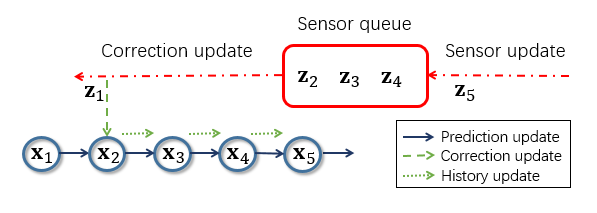
\includegraphics[width=0.7\textwidth]{Delayed and out-of-order measurement update.png}
	\bicaption{延时更新处理机制}{Delayed measurement handling mechanism.}
	\label{fig:Delayedmeasurementupdate}
\end{figure} 

$z_1$作为最旧的状态,首先输入到观测器上。$z_2$、$z_3$、$z_4$临时存储在队列中。根据传感器的延时$z_1$用于修正$x_2$的状态,然后向前更新历史状态。最新的状态$x_5$则通过最新的IMU数据进行预测更新。

\gdutsubsection{我们的算法实现}{Implementation of our algorithm}
为了验证所提出的传感器融合算法,我们开发了一个具有多个传感器的四旋翼飞行器平台。该平台在第1.3节中进行了讨论,如所示。实验平台是我们自行组装的平台。该平台包含一个飞控板,由IMU和一个STM32微控制器组成。其中陀螺仪的采样频率为2000Hz,加速度计的采样频率为800Hz。

\autoref{fig:stateestimation}为平台的传感器配置。注意,根据任务需求和实际情况,可以直接添加或删除传感器。我们开发的程序流程如(\autoref{fig:Flowchartoffusionalgorithm})。本节将介绍了改进后算法的具体实现。
\begin{figure}[htbp]
	\centering
	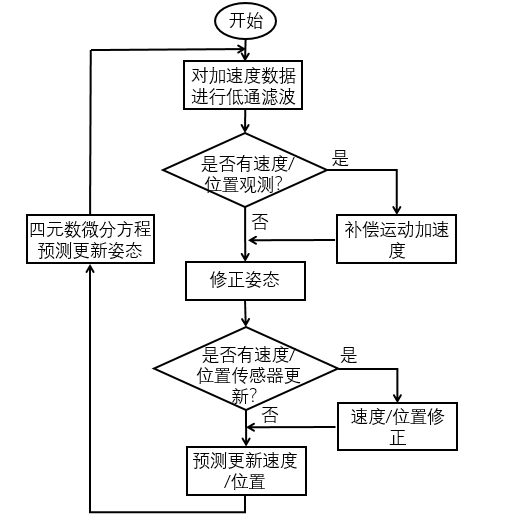
\includegraphics[width=0.6\textwidth]{屏幕截图 2022-03-06 210135.png}
	\bicaption{融合算法流程图}{Flow chart of fusion algorithm}
	\label{fig:Flowchartoffusionalgorithm}
\end{figure}

由于陀螺仪的采样频率和加速度计的采样频率不一致,我们将姿态预测和姿态修正分离,只要陀螺仪数据更新,我们就根据四元数微分方程使用角速度数据进行积分。
\begin{equation}\label{eq:quatint}
		\dot{q}(k)=\frac{1}{2} q \otimes \mathbf{p}(\Omega_y(k))
\end{equation}

对于加速度计来说,某些构型的飞行器机身可产生10个重力加速度大小的震动,加速度计对震动非常敏感,飞行过程中姿态的真实信息被震动加速度淹没了。针对震动噪声的问题,一般的解决方案是对加速度的数据进行一个低截止频率的低通滤波。

上小节提到,我们使用观测器-预测器方法对历史状态处理,文\cite{khosravian2014velocity}在机体系下求出历史误差,没有历史状态进行修正。使用机体系下的误差对历史状态修正在实际应用中并不准确。原因是每个历史状态的机体系都是不一样的,不同坐标系的向量无法进行运算。我们使用在世界系求姿态误差,然后对历史状态进行修正。此外,由GPS差分的运动加速度和IMU的更新频率不一致,我们用线性插值计算运动加速度作补偿。设计如下观测器:
\begin{equation}\label{eq:myrpcorrection}
	\begin{aligned}
		\Delta a &= \frac{v - v_{last}}{\Delta t}\\
		a_m (k-d) &= a_{mlast} + \frac{k-d}{k-k_{last}} \Delta a\\
		a_{ref} (k-d) &= a_m (k-d) + g e_3\\
		\sigma &= k_a \hat{R}(k-d) a(k-d) \times a_{ref}(k-d)\\
		q_{correction}^{RP} &= \mathbf{p}(\sigma)\\
		\hat{q}(k-n) &= q_{correction}^{RP} \otimes \hat{q}(k-n)
	\end{aligned}
\end{equation}
其中,$a_m (t-d)$为$k-d$时刻通过插值计算的运动加速度,$\hat{R}(k-d)$为$k-d$时刻的姿态,$\sigma$为$k-d$时刻的修正量。我们使用$k-d$时刻的误差修正当前状态。

同理,根据我们在上一节对偏航解耦的分析,对磁力计/GPS的延时处理,设计如下观测器:
\begin{equation}\label{eq:myyawcorrection}
	\begin{aligned}
		\sigma &= k_y (\psi_{mag/gps}(k-d) - \hat{\psi}(k-d)) \\
		q_{correction}^{Y} &= \begin{bmatrix}
			cos(\frac{\sigma}{2}) \\
			0 \\
			0 \\
			sin(\frac{\sigma}{2})
		\end{bmatrix}\\
		\hat{q}(k-n) &= q_{correction}^{Y} \otimes \hat{q}(k-n)
	\end{aligned}
\end{equation}
其中,$\psi_{mag/gps}(k-d)$为$k-d$时刻由磁力计/GPS就算的偏航角,$d$可以根据传感器不同更改。

和姿态估计类似,位置速度估计也可以分为预测和修正两部分,只要加速度数据更新,我们就使用加速度数据进行积分。
\begin{equation}\label{eq:pvpredict}
	\begin{aligned}
		a^W(k) &= \hat{R}_B^W a^B(k) - g e_3\\
		v(k) &= v(k-1) + a^W(k) \Delta t\\
		p(k) &= p(k-1) + v(k) \Delta t
	\end{aligned}
\end{equation}
其中$\Delta t$是步长。

同理,仿照\autoref{eq:pvpredict}中的延时补偿方法,我们有位置速度观测器:
\begin{equation}\label{eq:mypvcorrection}
	\begin{aligned}
		\hat{v}(k-n) &= \hat{v}(k-n) + k_v (v_m(k-d) - \hat{v}(k-d))\\
		\hat{p}(k-n) &= \hat{p}(k-n) + k_p (p_m(k-d) - \hat{p}(k-d))
	\end{aligned}
\end{equation}
取$n=0,1,...,d$修正$k-d$时刻到$k$时刻的历史状态。

\gdutsection{实验结果}{Experimental results}
我们通过飞行实验验证了系统的鲁棒性。在实验中,飞行器都是通过使用其板载状态估计作为反馈进行自主控制。我们使用RTK对估计器进行定量评估。实验平台的介绍在第一章。控制方法的介绍在第四章。

\gdutsubsection{评估估计器的性能}{Evaluating estimator performance}
我们希望通过与真值对比以研究估计器的性能,真值是由厘米级精确度的GPS/RTK系统定义的。在飞行器飞行时,本实验通过比较板载估计器输出与的GPS/RTK来评估估计的准确性。下面,我们给出RTK和板载估计的标准差。roll和pitch使用运动加速度评估,运动加速度的标准差为$\big\{ \sigma_{a_x},\sigma_{a_y} \big\}=\big\{ 22.61, 17.28 \big\}$(cm/s)。yaw的标准差为$\sigma_{\psi}=6.36$(deg)。位置的标准差为$\big\{ \sigma_{p_x},\sigma_{p_y},\sigma_{p_z} \big\}=\big\{ 3.21, 1.37, 1.44 \big\}$(cm)。速度的标准差为$\big\{ \sigma_{v_x},\sigma_{v_y},\sigma_{v_z} \big\}=\big\{ 3.37, 3.31, 4.26 \big\}$(cm/s)。

\gdutsubsection{飞行器飞行实验}{UAV flying test}
在本实验中,我们让飞行器沿约100米长的直线轨迹飞行,最大速度为5m/s。性能是根据来自RTK的真值进行评估的。估计的轨迹、位置、速度和姿态如所示。在图中可以看到较大且频繁的姿态变化。

我们的目标是生成适合高速飞行的状态估计。我们可以看到,估计速度与真值的速度吻合得很好。

\gdutsection{总结与讨论}{Summary and discussion}
在本章中,我们展示了使用IMU作为主要传感器,融合其他传感器进行状态估计以实现飞行器的稳定飞行。关键技术是考虑了传感器延时,运动加速度补偿以及异常处理相关的算法。此外,我们将容易受到磁场干扰的偏航角和俯仰、横滚角解耦以保证系统的鲁棒性。本文提出的算法可以使飞行器保持稳定。

\gdutchapter{传感器校准}{Sensor calibration}
在本章中,我们研究如何使用较少的仪器来进行高精度的传感器校准以提供更好的传感器数据。一般来说,基于MEMS的传感器的精度都比较差,远远达不到高精度导航的要求。然而,开发基于MEMS的传感器的飞行器,要保证传感器数据精度是很困难的。在本章中,我们研究传感器校准算法,开发了一种不需要外部设备就可以进行较高精度的校准。我们详细介绍了基于优化的传感器校准算法,并将其与融合和控制方法(第4章)结合起来进行实验,以验证系统的性能。

本系统的关键技术是一种传感器校准算法,能够无需外部设备的情况下进行校准。我们要求校准算法能够使用人手就能完成,无需外部设备,在尽量简单的校准流程下保证校准结果的准确性。

\gdutsection{加速度计校准}{Acceleromter calibration}
首先建立加速度计的传感器模型,并利用重力的向量大小进行标定\cite{jekeli2012inertial}。对于加速度计,我们使用静态检测的方法\cite{fong2008methods},并使用基于方差的检测算法\cite{sabatini2006wavelet}。由于需要提取静止的重力向量,我们可以对原始数据进行静态检测,放宽校准种严格的静止的条件。利用校准后的参数将原始数据转化为标准的重力向量$g$。

我们的检测器基于基于Tedaldi的方法:对于每个加速度计样本$\begin{bmatrix}
	a^t_x & a^t_y & a^t_z
\end{bmatrix}$,给定一个长度为t秒的时间间隔时刻,我们计算方差的大小
\begin{equation}\label{eq:var}
	\zeta(t)=\sqrt{[var_{t_w}(a^t_x)]^2+[var_{t_w}(a^t_y)]^2+[var_{t_w}(a^t_z)]^2}
\end{equation}
其中$var_{t_w}(a^t)$是一个运算符,计算加速度计$a^t$在以$t$为中心,长度为$t_w$秒的时间间隔内的方差。我们通过判断$\zeta(t)$是否小于或大于一个阈值对静态和运动间隔进行分割。与传统的六面校准法相比\cite{尹杭2014一种},该方法在可以在任意姿态下保持静止。

\gdutsubsection{传感器误差模型}{Sensor error model}
对于加速度计,有
\begin{equation}\label{eq:axiserror}
	T^{a}=
	\begin{bmatrix}
		1 & \beta_{yz} & \beta_{zy}\\
		\beta_{xz} & 1 & \beta_{zx}\\
		\beta_{xy} & \beta_{yx} & 1
	\end{bmatrix}
\end{equation}
其中,$T^a$是轴正交矩阵,$\beta_{ij}$是第$i$个传感器轴的误差对第$j$个轴的造成的误差影响。

此外,加速度计受到零偏和尺度误差的影响。引入尺度矩阵
\begin{equation}\label{eq:scaleerror}
	K^{a}=
	\begin{bmatrix}
		s^a_x & 0 & 0\\
		0 & s^a_y & 0\\
		0 & 0 & s^a_z
	\end{bmatrix}
\end{equation}
我们接着引入零偏向量
\begin{equation}\label{eq:scaleerror}
	b^{a}=
	\begin{bmatrix}
		b^a_x\\
		b^a_y\\
		b^a_z
	\end{bmatrix}
\end{equation}
完整的传感器误差模型为
\begin{equation}\label{eq:sensorerrormodel}
	a^O=T^a K^a (a^S + b^a + \nu^a)
\end{equation}
其中,$a^O$和$a^S$分别表示校准后和校准前的加速度数据,$ν^a$是加速度计测量噪声。

\gdutsection{陀螺仪校准}{Gyroscope calibration}
一般来说,对于陀螺仪校准,要完整校准出零偏、尺度和轴正交要比加速度计校准复杂得多。即使对角速度精度有较高得要求,由于缺乏相应的设备,也无法校准出陀螺仪的尺度和轴正交参数。简单的陀螺校准无法用于高精度的导航上。因此,基于Tedaldi的方法\cite{tedaldi2014robust},我们将对陀螺仪进行十二参数的标定。

\gdutsection{磁力计校准}{Magnetometer calibration}
磁力计本身的系统误差非常大,直接用原始数据计算偏航角的精度十分差以至于无法用于控制飞行器的偏航。因此,我们基于椭球拟合的方法来校准磁力计\cite{李勇2012基于椭球拟合的三轴磁传感器误差补偿方法}。我们使用牛顿迭代法求解最小二乘问题,因为代价函数是非线性的。传感器测量模型与章节3.1相同。

\gdutsection{实验结果}{Experimental results}
实验环境不需要任何外部设备。在所有的实验中,我们只需要采集传感器的原始数据。实验平台在第1章中进行了讨论。实验平台是基于开源飞控。这个现成的飞控板配有一个IMU、一个磁力计和一个STM32微控制器。

\gdutsubsection{加速度计校准结果}{Accelrometer calibration result}
在本实验中,采集IMU原始数据,使其以任意姿态静止。整个校准流程为3分钟。校准精度是根据重力模长进行评估的。加速度计校准结果显示在。

\gdutsubsection{陀螺仪校准结果}{Gyroscope calibration result}
这个实验给出陀螺校准结果。陀螺仪和加速度计同时校准。校准精度是根据角度误差来评估的。陀螺仪校准结果显示在。

\gdutsubsection{磁力计校准结果}{Magnetometer calibration result}
在本实验中,采集磁力计原始数据,以足够多的姿态运动飞控。校准精度根据磁场模长进行评估。磁力计校准结果显示在。

\gdutsection{总结与讨论}{Summary and discussion}
在本章中,我们提出了一种IMU校准算法,该方法能够在无需外部设备的情况下进行校准。我们对校准评估标准方法的进行优化。我们的方法能够使精度提高到xxx。

\gdutchapter{控制}{Control methods}
本章讨论如何调整控制方法,以配合飞行器稳定飞行的需要。我们介绍了保证状态估计和控制平滑的系统体系结构。

\gdutsection{反馈控制}{Feedback control}
在给定估计的状态后,我们让飞行器用位置跟踪控制器来跟踪所需的轨迹\cite{lee2010geometric}。由传感器融合模块(第二章)的状态估计直接作为控制器的反馈。在本文的设计中,姿态控制器和位置控制器都在STM32以400Hz的频率运行。

\gdutsection{实验结果}{Experimental results}
我们有一个基于多传感器融合的状态估计器来产生800Hz的位置、速度、姿态估计,足以稳定飞行器。

在这个实验中,飞行器以大约1米/秒的速度自动沿着矩形轨迹生成平滑轨迹。使用GPS/RTK在信号良好的状态下来量化全局跟踪性能。由图xxx可以看出,飞行器的实际位置收敛到期望位置,其标准差为xxx,表明控制器的稳定收敛。

\gdutbackmatter
\gdutchapter{结论与展望}{Conclusion and prospect}
在这篇论文中,我们展示了对飞行器自主飞行的最新技术的贡献,大部分贡献是状态估计算法。在第三章中,我们开发了状态估计系统,提出了一种模块化和可扩展的方法,该方法能够以一致的方式组合来自多个传感器的信息。在第四章中,我们开发了传感器校准算法,能够在没有外部设备的情况下对传感器进行高精度的校准。在第五章中,我们提出的控制方法结合前两章的算法形成一个集成的飞行器系统。

我们注意到,虽然主要的实验平台使用的是四旋翼,但我们的方法不限于这一特定类型的平台。实际上,我们的方法是基于传感器的,同样适用于其他机器人,如固定翼、地面机器人等。
\gdutbacksection{成果总结}
综上所述,本文的主要贡献如下:
\begin{itemize}
	\item 我们开发了算法和系统,使计算资源受限的飞行器能够自主飞行,只使用低成本的传感器。
	\item 我们提出了一种算法,通过互补融合来自多传感器的信息来提高系统的可靠性。
	\item 我们提出了一种算法,无需外部设备就能够进行传感器校准。
	\item 我们开发集成了控制算法,并通过大量的实验表明,飞行控制系统是稳定可靠的。
\end{itemize}

\gdutbacksection{未来研究展望}
本文涉及到了几个有趣的研究领域,其中一些是随着飞行器技术的发展而不断发展成大型系统的,而另一些则是我们在评估最新方法的性能时值得追求的新方向。
\paragraph{自主飞行中估计与控制的耦合设计。}
在我们目前的工作中,控制器与估计器是分开设计的。然而,随着我们朝着高速自主飞行的方向发展,我们可能会要求估计器和控制器耦合设计,以生成和执行高效、无碰撞和安全的飞行轨迹。
\paragraph{用于飞行器的新的传感器技术。}
虽然传统的传感器如IMU、GPS、相机已被证明可用于飞行器导航,但最近传感技术的发展可能创造新的机会。例如,光场可以作为深度感知的传感器。这些新型传感技术在飞行器上的应用具有很大的潜力。
\paragraph{传感器和能观性研究。}
众所周知,传感器数量越多,系统的能观性越好,但单个传感器对系统能观性的影响尚不清楚。增加更多的传感器会带来出更多的能观性,但是传感器提供的信息以及信息的质量会导致能观性的复杂判断条件。因此,一个能够以在线方式识别能观性的通用框架将有利于更高层次的任务,如运动规划和风险评估。

\nocite{*}% 列出全部参考文献
\printbibliography

\gdutchapter{攻读学位期间取得与学位论文相关的成果}{Publication and patents during study}

\gdutbacksection{发表和投稿与学位论文相关学术论文}

\begin{results}
  \item \textbf{张三}, 李四, 等. Jet electrochemical machining of micro dimples with conductive mask.
  Journal of Materials Processing Technology. 2018, 257:101-111. (SCI Impact Factor 3.647,
  WOS:000431161400010)
  \item 李四, \textbf{张三}, 王五, 等. Electrochemical direct-writing machining of micro- channel array.
  Journal of Materials Processing Technology. 2019, 265:138-149. (SCI Impact Factor 3.647,
  WOS:000451935100014)
\end{results}

\gdutbacksection{申请发明专利}

\begin{results}
  \item 李四, \textbf{张三}, 王五. 一种微流道电解加工装置. 发明专利申请号: 201810467763.5.
\end{results}

\gdutstatement

\gdutchapter{致谢}{Acknowlegements}
\zhlipsum[1]

\gdutappendix

\gdutchapter{附录标题}{The appendix title}
对需要收录于学位论文中且又不适合书写于正文中的附加数据、资料、详细
公式推导、计算机程序等有特色的内容,可做为附录排写。
\end{document}